\documentclass[12pt, letterpaper]{article}
\usepackage[utf8]{inputenc}
\usepackage{amsmath}
\usepackage{graphicx}
\graphicspath{{images/}}

\title{AI1110 Assignment 1}
\author{Tejal Kulkarni CS21BTECH11058}
\date{March 2022}

\begin{document}
\maketitle

\section*{Q8(c)}
    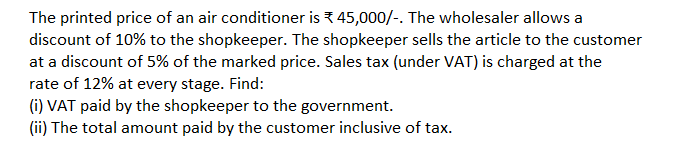
\includegraphics[scale=1.10]{question.png}
    \section*{Solution:}
Marked  Price = Rs.45,000/- \\
Sales  Tax = 12\% \\
Discount  for  shopkeeper = 10\% \\ \\
Discount  amount for shopkeeper =  \begin{equation*}
    45000\times\frac{10}{100} = Rs.4500\\ 
    \end{equation*} 
Selling Price for shopkeeper = \begin{equation*}
    45000 - 4500 = Rs.40500 \\
\end{equation*}
Sales Tax for shopkeeper = \begin{equation*} \\
    40500\times\frac{12}{100} =  Rs.4860\\
\end{equation*}
Discount for customer = 5\% \\ \\
Discount amount for customer  = 
\begin{equation*} 
     45000\times\frac{5}{100} = Rs.2250 \\ 
    \end{equation*}
Selling Price for customer = \begin{equation*}\\
    45000 - 2250 =  Rs.42750\\
\end{equation*}
Sales tax for customer = \begin{equation*}\\
    42750\times\frac{12}{100} = Rs.5130\\
\end{equation*} \\
Hence,\\
i) VAT paid by shopkeeper to government = \\
    \begin{equation*}
       5130 - 4860 = Rs.270\\
   \end{equation*}
ii) Total Amount paid by customer = \\
    \begin{equation*}
       42750 + 5130 = Rs.47880\\
   \end{equation*} \\ \\
The output of the program used for verification:\\ \\
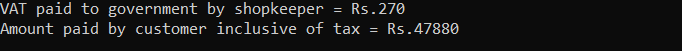
\includegraphics[scale=1.1]{codeoutput.png} \\

\end{document}
